\documentclass{beamer}

\beamertemplatenavigationsymbolsempty % Retire les symboles de navigations en bas a droite
\setbeamertemplate{footline}[frame number]

\usepackage{graphicx}
\graphicspath{ {Images} }

\usetheme{Hannover}
\usecolortheme{seahorse}
\logo{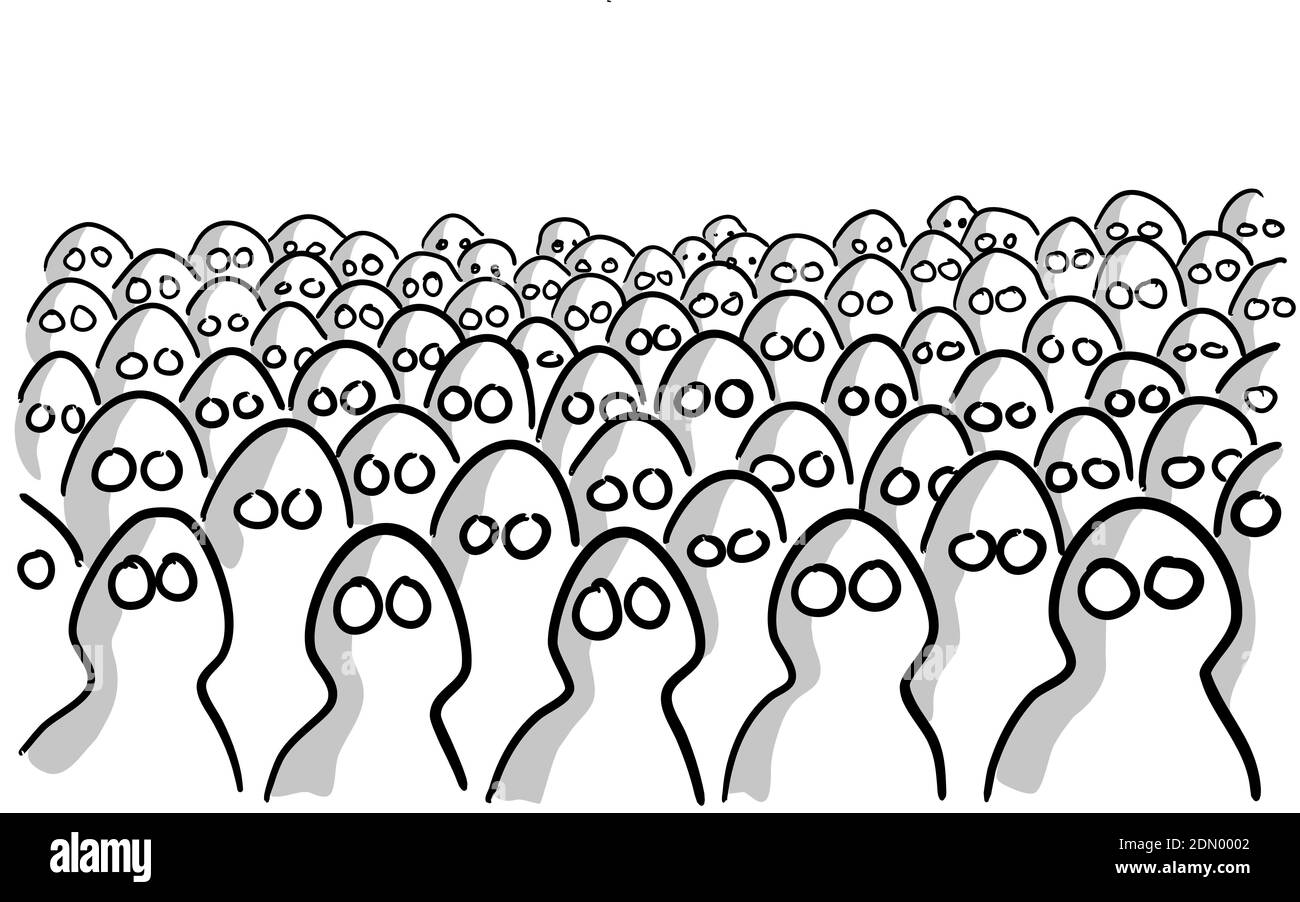
\includegraphics[height=1cm ]{logo.jpg}}

\title{Optimisation d’un batiment dans le cadre
d’une évacuation d’urgence}
\author{Clodion Thibault n°00000}
\date{Présentation TIPE - La Ville}


\begin{document}

\frame{\titlepage} % Slide n°1 avec le titre etc

\begin{frame}{Table des matières}
    \tableofcontents
\end{frame}

\section{Introduction}

\subsection{Enjeu}

\begin{frame}
    Exemple de Frame
\end{frame}

\subsection{Exemple}

\section{Modélisation de la Foule}
\subsection{L'algorithme}
\subsection{Amélioration du réalisme et choix}

\section{Optimisation du Bâtiment}
\subsection{Bâtiment et normes}
\subsection{Processus d'optimisation}
\subsection{Résultat}

\section{Influence des paramètres sur le bâtiment}
\subsection{Ajout de porte}
\subsection{Taille porte}
\subsection{e}
\subsection{e}


\begin{frame}
    % Force l'apparition de la table des matières
\end{frame}

\end{document}